\begin{solution}
\begin{enumerate}
\item {[4 points]} If $v\in\{w\in C^2[0,1]:w(1)=0\}$, then
\[
-\int_0^1u''(x)v(x)\,dx=(f,v).
\]
Integration by parts then yields that
\[
-[u'(x)v(x)]_0^1+a(u,v)=(f,v)
\]
from which we can conclude that
\[
\alpha v(0)+a(u,v)=(f,v)
\]
since $v(1)=0$ and $u'(0)=\alpha$. Therefore,
\[
a(u,v)=g(f,\alpha,v)\mbox{ for all }v\in\{w\in C^2[0,1]:w(1)=0\}
\]
where
\[
g(f,\alpha,v)=(f,v)-\alpha v(0).
\]

\vspace*{1em}
\item {[8 points]} The plot and code used to create it, and the plot shown in part (c), are below. Note that the below code uses the MATLAB function which you had to write in Homework 2.

\begin{center}
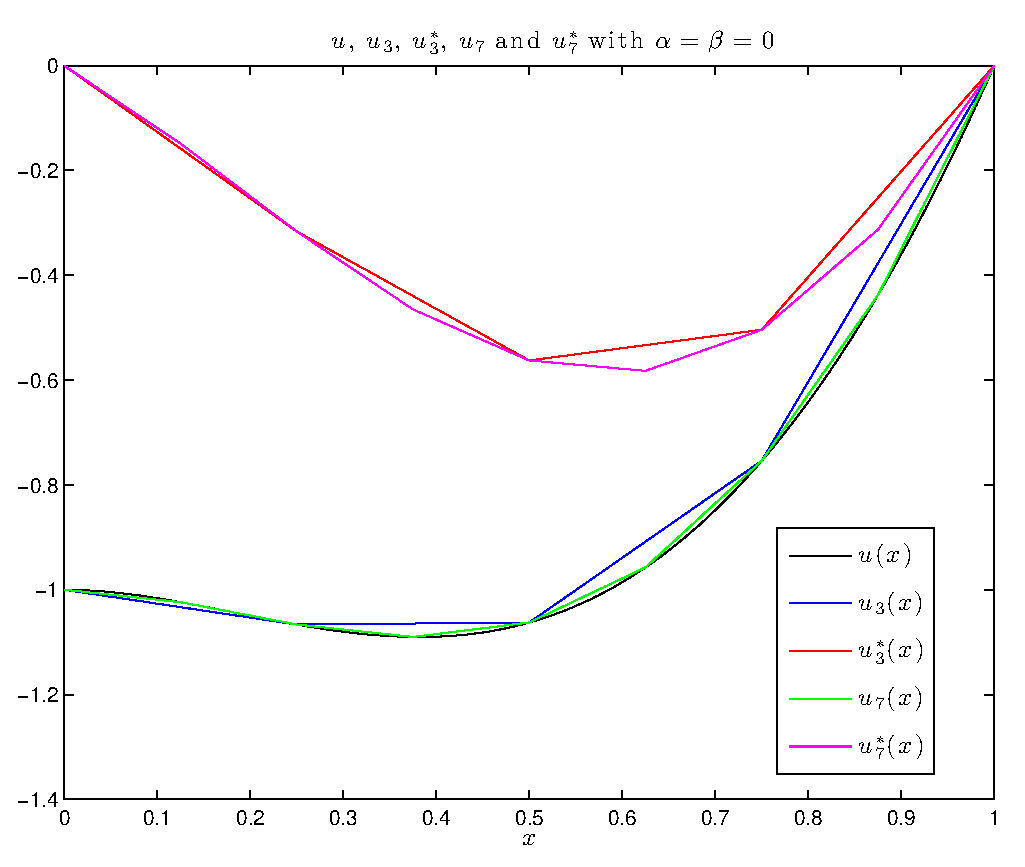
\includegraphics[scale=0.7]{hw37c.eps}
\end{center}

\lstinputlisting{HW37cd.m}

\vspace*{1em}
\item {[6 points]} The plot is below.

\begin{center}
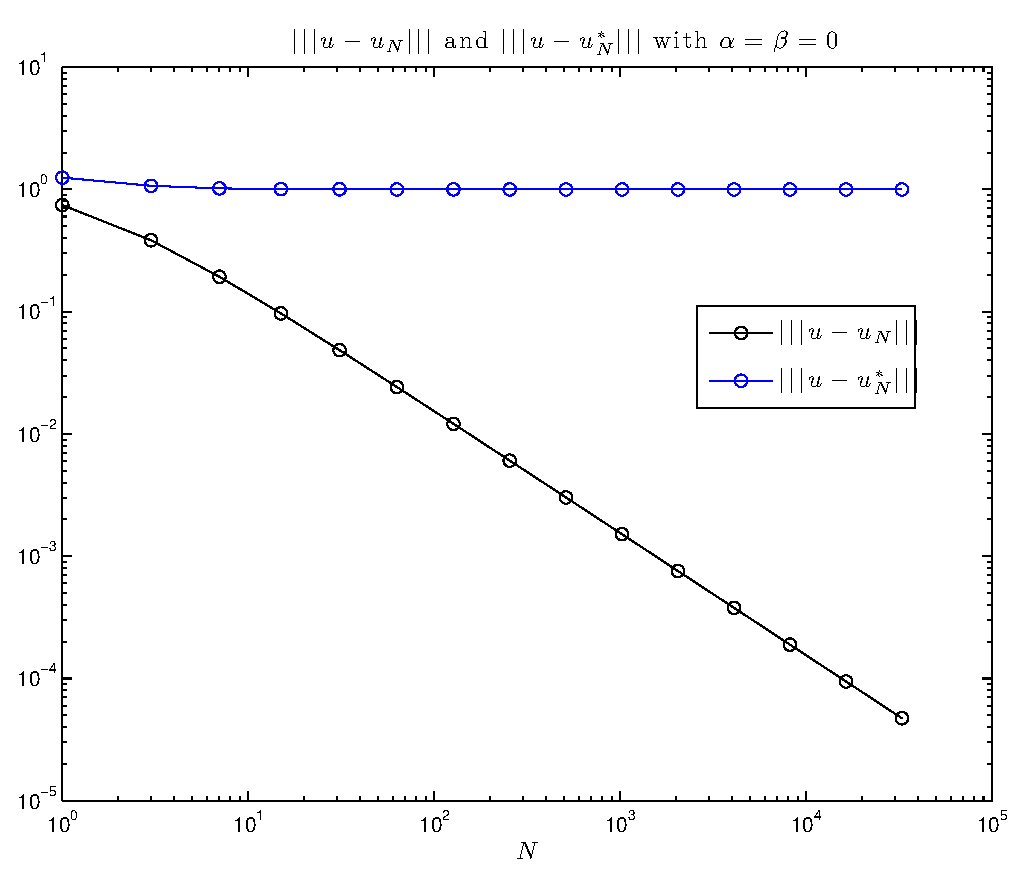
\includegraphics[scale=0.7]{hw37d.eps}
\end{center}

\vspace*{1em}
\item {[7 points]} The plot and code used to create it are below. Note that the below code uses the MATLAB function which you had to write in Homework 2.

\begin{center}
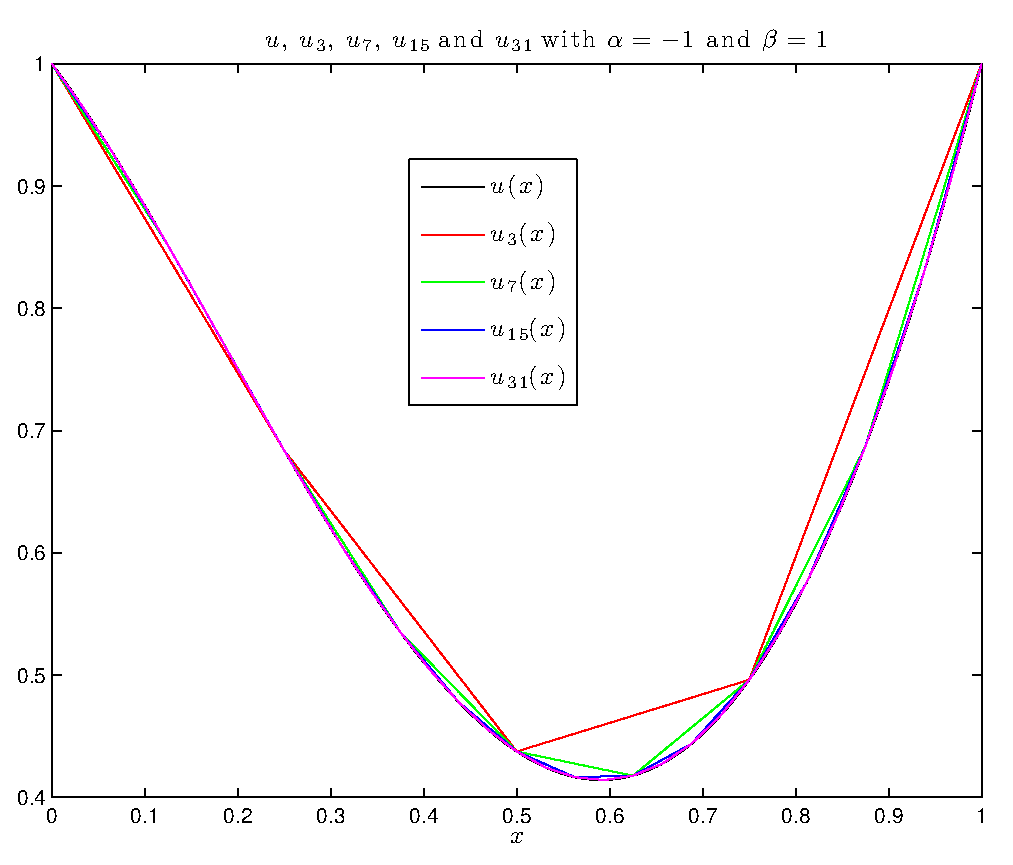
\includegraphics[scale=0.7]{hw37e.eps}
\end{center}

\lstinputlisting{HW37e.m}

\end{enumerate}
\end{solution}
